\documentclass[]{article}
\usepackage{lmodern}
\usepackage{amssymb,amsmath}
\usepackage{ifxetex,ifluatex}
\usepackage{fixltx2e} % provides \textsubscript
\ifnum 0\ifxetex 1\fi\ifluatex 1\fi=0 % if pdftex
  \usepackage[T1]{fontenc}
  \usepackage[utf8]{inputenc}
\else % if luatex or xelatex
  \ifxetex
    \usepackage{mathspec}
  \else
    \usepackage{fontspec}
  \fi
  \defaultfontfeatures{Ligatures=TeX,Scale=MatchLowercase}
\fi
% use upquote if available, for straight quotes in verbatim environments
\IfFileExists{upquote.sty}{\usepackage{upquote}}{}
% use microtype if available
\IfFileExists{microtype.sty}{%
\usepackage{microtype}
\UseMicrotypeSet[protrusion]{basicmath} % disable protrusion for tt fonts
}{}
\usepackage[margin=1in]{geometry}
\usepackage{hyperref}
\hypersetup{unicode=true,
            pdfborder={0 0 0},
            breaklinks=true}
\urlstyle{same}  % don't use monospace font for urls
\usepackage{color}
\usepackage{fancyvrb}
\newcommand{\VerbBar}{|}
\newcommand{\VERB}{\Verb[commandchars=\\\{\}]}
\DefineVerbatimEnvironment{Highlighting}{Verbatim}{commandchars=\\\{\}}
% Add ',fontsize=\small' for more characters per line
\usepackage{framed}
\definecolor{shadecolor}{RGB}{248,248,248}
\newenvironment{Shaded}{\begin{snugshade}}{\end{snugshade}}
\newcommand{\KeywordTok}[1]{\textcolor[rgb]{0.13,0.29,0.53}{\textbf{#1}}}
\newcommand{\DataTypeTok}[1]{\textcolor[rgb]{0.13,0.29,0.53}{#1}}
\newcommand{\DecValTok}[1]{\textcolor[rgb]{0.00,0.00,0.81}{#1}}
\newcommand{\BaseNTok}[1]{\textcolor[rgb]{0.00,0.00,0.81}{#1}}
\newcommand{\FloatTok}[1]{\textcolor[rgb]{0.00,0.00,0.81}{#1}}
\newcommand{\ConstantTok}[1]{\textcolor[rgb]{0.00,0.00,0.00}{#1}}
\newcommand{\CharTok}[1]{\textcolor[rgb]{0.31,0.60,0.02}{#1}}
\newcommand{\SpecialCharTok}[1]{\textcolor[rgb]{0.00,0.00,0.00}{#1}}
\newcommand{\StringTok}[1]{\textcolor[rgb]{0.31,0.60,0.02}{#1}}
\newcommand{\VerbatimStringTok}[1]{\textcolor[rgb]{0.31,0.60,0.02}{#1}}
\newcommand{\SpecialStringTok}[1]{\textcolor[rgb]{0.31,0.60,0.02}{#1}}
\newcommand{\ImportTok}[1]{#1}
\newcommand{\CommentTok}[1]{\textcolor[rgb]{0.56,0.35,0.01}{\textit{#1}}}
\newcommand{\DocumentationTok}[1]{\textcolor[rgb]{0.56,0.35,0.01}{\textbf{\textit{#1}}}}
\newcommand{\AnnotationTok}[1]{\textcolor[rgb]{0.56,0.35,0.01}{\textbf{\textit{#1}}}}
\newcommand{\CommentVarTok}[1]{\textcolor[rgb]{0.56,0.35,0.01}{\textbf{\textit{#1}}}}
\newcommand{\OtherTok}[1]{\textcolor[rgb]{0.56,0.35,0.01}{#1}}
\newcommand{\FunctionTok}[1]{\textcolor[rgb]{0.00,0.00,0.00}{#1}}
\newcommand{\VariableTok}[1]{\textcolor[rgb]{0.00,0.00,0.00}{#1}}
\newcommand{\ControlFlowTok}[1]{\textcolor[rgb]{0.13,0.29,0.53}{\textbf{#1}}}
\newcommand{\OperatorTok}[1]{\textcolor[rgb]{0.81,0.36,0.00}{\textbf{#1}}}
\newcommand{\BuiltInTok}[1]{#1}
\newcommand{\ExtensionTok}[1]{#1}
\newcommand{\PreprocessorTok}[1]{\textcolor[rgb]{0.56,0.35,0.01}{\textit{#1}}}
\newcommand{\AttributeTok}[1]{\textcolor[rgb]{0.77,0.63,0.00}{#1}}
\newcommand{\RegionMarkerTok}[1]{#1}
\newcommand{\InformationTok}[1]{\textcolor[rgb]{0.56,0.35,0.01}{\textbf{\textit{#1}}}}
\newcommand{\WarningTok}[1]{\textcolor[rgb]{0.56,0.35,0.01}{\textbf{\textit{#1}}}}
\newcommand{\AlertTok}[1]{\textcolor[rgb]{0.94,0.16,0.16}{#1}}
\newcommand{\ErrorTok}[1]{\textcolor[rgb]{0.64,0.00,0.00}{\textbf{#1}}}
\newcommand{\NormalTok}[1]{#1}
\usepackage{graphicx,grffile}
\makeatletter
\def\maxwidth{\ifdim\Gin@nat@width>\linewidth\linewidth\else\Gin@nat@width\fi}
\def\maxheight{\ifdim\Gin@nat@height>\textheight\textheight\else\Gin@nat@height\fi}
\makeatother
% Scale images if necessary, so that they will not overflow the page
% margins by default, and it is still possible to overwrite the defaults
% using explicit options in \includegraphics[width, height, ...]{}
\setkeys{Gin}{width=\maxwidth,height=\maxheight,keepaspectratio}
\IfFileExists{parskip.sty}{%
\usepackage{parskip}
}{% else
\setlength{\parindent}{0pt}
\setlength{\parskip}{6pt plus 2pt minus 1pt}
}
\setlength{\emergencystretch}{3em}  % prevent overfull lines
\providecommand{\tightlist}{%
  \setlength{\itemsep}{0pt}\setlength{\parskip}{0pt}}
\setcounter{secnumdepth}{0}
% Redefines (sub)paragraphs to behave more like sections
\ifx\paragraph\undefined\else
\let\oldparagraph\paragraph
\renewcommand{\paragraph}[1]{\oldparagraph{#1}\mbox{}}
\fi
\ifx\subparagraph\undefined\else
\let\oldsubparagraph\subparagraph
\renewcommand{\subparagraph}[1]{\oldsubparagraph{#1}\mbox{}}
\fi

%%% Use protect on footnotes to avoid problems with footnotes in titles
\let\rmarkdownfootnote\footnote%
\def\footnote{\protect\rmarkdownfootnote}

%%% Change title format to be more compact
\usepackage{titling}

% Create subtitle command for use in maketitle
\newcommand{\subtitle}[1]{
  \posttitle{
    \begin{center}\large#1\end{center}
    }
}

\setlength{\droptitle}{-2em}

  \title{}
    \pretitle{\vspace{\droptitle}}
  \posttitle{}
    \author{}
    \preauthor{}\postauthor{}
    \date{}
    \predate{}\postdate{}
  

\begin{document}

\subsection{Validation of effect size estimates for One-Way
ANOVA}\label{validation-of-effect-size-estimates-for-one-way-anova}

We first repeat the simulation by Brysbaert:

\begin{Shaded}
\begin{Highlighting}[]
\CommentTok{# Simulations to estimate the power of an ANOVA with three unrelated groups}
\CommentTok{# the effect between the two extreme groups is set to d = .4, the effect for the third group is d = .4 (see below for other situations)}
\CommentTok{# we use the built-in aov-test command}

\CommentTok{# give sample sizes (all samples sizes are equal)}
\NormalTok{N =}\StringTok{ }\DecValTok{90}

\CommentTok{# give effect size d}
\NormalTok{d1 =}\StringTok{ }\FloatTok{.4} \CommentTok{#difference between the extremes}
\NormalTok{d2 =}\StringTok{ }\FloatTok{.4} \CommentTok{#third condition goes with the highest extreme}

\CommentTok{# give number of simulations}
\NormalTok{nSim =}\StringTok{ }\NormalTok{nsims}

\CommentTok{# give alpha levels}
\NormalTok{alpha1 =}\StringTok{ }\FloatTok{.05} \CommentTok{#alpha level for the omnibus ANOVA}
\NormalTok{alpha2 =}\StringTok{ }\FloatTok{.05} \CommentTok{#alpha level for three post hoc one-tailed t-tests Bonferroni correction}

\CommentTok{# create progress bar in case it takes a while}
\CommentTok{#pb <- winProgressBar(title = "progress bar", min = 0, max = nSim, width = 300)}

\CommentTok{# create vectors to store p-values}
\NormalTok{p1 <-}\KeywordTok{numeric}\NormalTok{(nSim) }\CommentTok{#p-value omnibus ANOVA}
\NormalTok{p2 <-}\KeywordTok{numeric}\NormalTok{(nSim) }\CommentTok{#p-value first post hoc test}
\NormalTok{p3 <-}\KeywordTok{numeric}\NormalTok{(nSim) }\CommentTok{#p-value second post hoc test}
\NormalTok{p4 <-}\KeywordTok{numeric}\NormalTok{(nSim) }\CommentTok{#p-value third post hoc test}
\NormalTok{pes1 <-}\KeywordTok{numeric}\NormalTok{(nSim) }\CommentTok{#partial eta-squared}
\NormalTok{pes2 <-}\KeywordTok{numeric}\NormalTok{(nSim) }\CommentTok{#partial eta-squared two extreme conditions}


\KeywordTok{library}\NormalTok{(lsr)}

\ControlFlowTok{for}\NormalTok{(i }\ControlFlowTok{in} \DecValTok{1}\OperatorTok{:}\NormalTok{nSim)\{ }\CommentTok{#for each simulated experiment}
 \CommentTok{# setWinProgressBar(pb, i, title=paste(round(i/nSim*100, 1), "% done"))}
\NormalTok{  x<-}\KeywordTok{rnorm}\NormalTok{(}\DataTypeTok{n =}\NormalTok{ N, }\DataTypeTok{mean =} \DecValTok{0}\NormalTok{, }\DataTypeTok{sd =} \DecValTok{1}\NormalTok{)}
\NormalTok{  y<-}\KeywordTok{rnorm}\NormalTok{(}\DataTypeTok{n =}\NormalTok{ N, }\DataTypeTok{mean =}\NormalTok{ d1, }\DataTypeTok{sd =} \DecValTok{1}\NormalTok{) }
\NormalTok{  z<-}\KeywordTok{rnorm}\NormalTok{(}\DataTypeTok{n =}\NormalTok{ N, }\DataTypeTok{mean =}\NormalTok{ d2, }\DataTypeTok{sd =} \DecValTok{1}\NormalTok{) }
\NormalTok{  data =}\StringTok{ }\KeywordTok{c}\NormalTok{(x,y,z)}
\NormalTok{  groups=}\StringTok{ }\KeywordTok{factor}\NormalTok{(}\KeywordTok{rep}\NormalTok{(letters[}\DecValTok{24}\OperatorTok{:}\DecValTok{26}\NormalTok{], }\DataTypeTok{each =}\NormalTok{ N))}
\NormalTok{  test <-}\StringTok{ }\KeywordTok{aov}\NormalTok{(data}\OperatorTok{~}\NormalTok{groups)}
\NormalTok{  pes1[i] <-}\StringTok{ }\KeywordTok{etaSquared}\NormalTok{(test)[}\DecValTok{1}\NormalTok{,}\DecValTok{2}\NormalTok{]}
\NormalTok{  p1[i] <-}\StringTok{ }\KeywordTok{summary}\NormalTok{(test)[[}\DecValTok{1}\NormalTok{]][[}\StringTok{"Pr(>F)"}\NormalTok{]][[}\DecValTok{1}\NormalTok{]]}
\NormalTok{  p2[i] <-}\StringTok{ }\KeywordTok{t.test}\NormalTok{(x,y)}\OperatorTok{$}\NormalTok{p.value}
\NormalTok{  p3[i] <-}\StringTok{ }\KeywordTok{t.test}\NormalTok{(x,z)}\OperatorTok{$}\NormalTok{p.value}
\NormalTok{  p4[i] <-}\StringTok{ }\KeywordTok{t.test}\NormalTok{(y,z)}\OperatorTok{$}\NormalTok{p.value}
\NormalTok{  data =}\StringTok{ }\KeywordTok{c}\NormalTok{(x,y)}
\NormalTok{  groups=}\StringTok{ }\KeywordTok{factor}\NormalTok{(}\KeywordTok{rep}\NormalTok{(letters[}\DecValTok{24}\OperatorTok{:}\DecValTok{25}\NormalTok{], }\DataTypeTok{each =}\NormalTok{ N))}
\NormalTok{  test <-}\StringTok{ }\KeywordTok{aov}\NormalTok{(data}\OperatorTok{~}\NormalTok{groups)}
\NormalTok{  pes2[i] <-}\StringTok{ }\KeywordTok{etaSquared}\NormalTok{(test)[}\DecValTok{1}\NormalTok{,}\DecValTok{2}\NormalTok{]}
\NormalTok{  \}}
\CommentTok{#close(pb)#close progress bar}

\CommentTok{# results are as predicted when omnibus ANOVA is significant, t-tests are significant between x and y plus x and z; not significant between y and z}
\CommentTok{#printing all unique tests (adjusted code by DL)}
\KeywordTok{sum}\NormalTok{(p1}\OperatorTok{<}\NormalTok{alpha1)}\OperatorTok{/}\NormalTok{nSim}
\end{Highlighting}
\end{Shaded}

\begin{verbatim}
## [1] 0.7932
\end{verbatim}

\begin{Shaded}
\begin{Highlighting}[]
\KeywordTok{sum}\NormalTok{(p2}\OperatorTok{<}\NormalTok{alpha2)}\OperatorTok{/}\NormalTok{nSim}
\end{Highlighting}
\end{Shaded}

\begin{verbatim}
## [1] 0.76073
\end{verbatim}

\begin{Shaded}
\begin{Highlighting}[]
\KeywordTok{sum}\NormalTok{(p3}\OperatorTok{<}\NormalTok{alpha2)}\OperatorTok{/}\NormalTok{nSim}
\end{Highlighting}
\end{Shaded}

\begin{verbatim}
## [1] 0.76014
\end{verbatim}

\begin{Shaded}
\begin{Highlighting}[]
\KeywordTok{sum}\NormalTok{(p4}\OperatorTok{<}\NormalTok{alpha2)}\OperatorTok{/}\NormalTok{nSim}
\end{Highlighting}
\end{Shaded}

\begin{verbatim}
## [1] 0.04968
\end{verbatim}

\begin{Shaded}
\begin{Highlighting}[]
\KeywordTok{mean}\NormalTok{(pes1)}
\end{Highlighting}
\end{Shaded}

\begin{verbatim}
## [1] 0.04140332
\end{verbatim}

\begin{Shaded}
\begin{Highlighting}[]
\KeywordTok{mean}\NormalTok{(pes2)}
\end{Highlighting}
\end{Shaded}

\begin{verbatim}
## [1] 0.04360753
\end{verbatim}

\subsection{Installation}\label{installation}

We install the functions:

\begin{Shaded}
\begin{Highlighting}[]
\CommentTok{# Install the two functions from GitHub by running the code below:}

\KeywordTok{source}\NormalTok{(}\StringTok{"https://raw.githubusercontent.com/Lakens/ANOVA_power_simulation/master/ANOVA_design.R"}\NormalTok{)}
\KeywordTok{source}\NormalTok{(}\StringTok{"https://raw.githubusercontent.com/Lakens/ANOVA_power_simulation/master/ANOVA_power.R"}\NormalTok{)}
\end{Highlighting}
\end{Shaded}

\subsection{Three conditions
replication}\label{three-conditions-replication}

\begin{Shaded}
\begin{Highlighting}[]
\NormalTok{K <-}\StringTok{ }\DecValTok{3}
\NormalTok{mu <-}\StringTok{ }\KeywordTok{c}\NormalTok{(}\DecValTok{0}\NormalTok{, }\FloatTok{0.4}\NormalTok{, }\FloatTok{0.4}\NormalTok{)}
\NormalTok{n <-}\StringTok{ }\DecValTok{90}
\NormalTok{sd <-}\StringTok{ }\DecValTok{1}
\NormalTok{r <-}\StringTok{ }\DecValTok{0}
\NormalTok{string =}\StringTok{ }\KeywordTok{paste}\NormalTok{(K,}\StringTok{"b"}\NormalTok{,}\DataTypeTok{sep=}\StringTok{""}\NormalTok{)}
\end{Highlighting}
\end{Shaded}

\begin{Shaded}
\begin{Highlighting}[]
\NormalTok{design_result <-}\StringTok{ }\KeywordTok{ANOVA_design}\NormalTok{(}\DataTypeTok{string =}\NormalTok{ string,}
                   \DataTypeTok{n =}\NormalTok{ n, }
                   \DataTypeTok{mu =}\NormalTok{ mu, }
                   \DataTypeTok{sd =}\NormalTok{ sd, }
                   \DataTypeTok{labelnames =} \KeywordTok{c}\NormalTok{(}\StringTok{"factor1"}\NormalTok{, }\StringTok{"level1"}\NormalTok{, }\StringTok{"level2"}\NormalTok{, }\StringTok{"level3"}\NormalTok{))}
\end{Highlighting}
\end{Shaded}

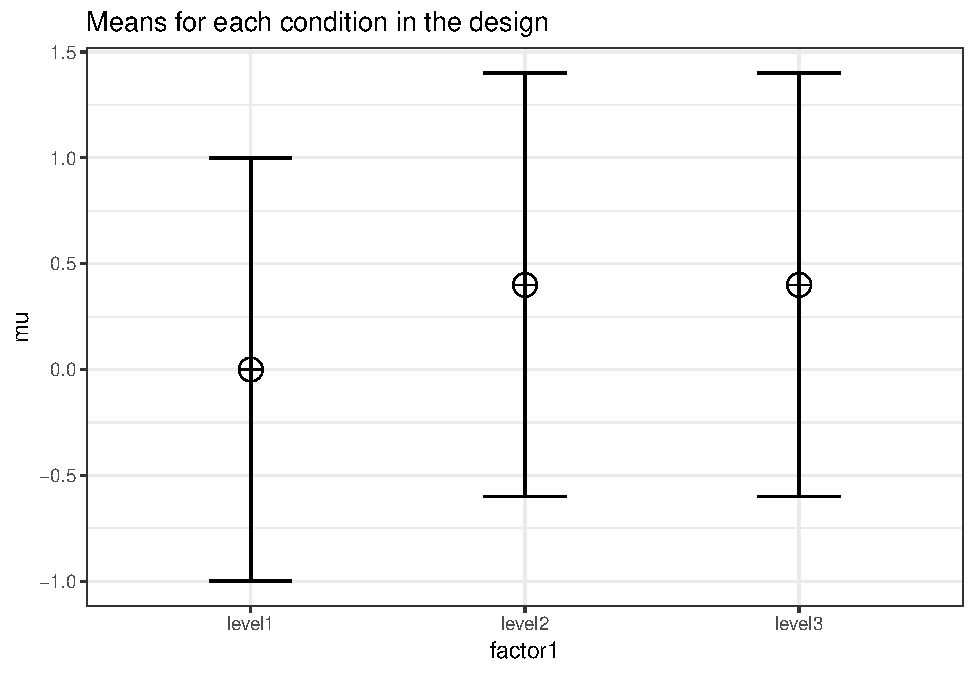
\includegraphics{1.3_validation_power_between_Brysbaert_1x3_files/figure-latex/unnamed-chunk-4-1.pdf}

\begin{Shaded}
\begin{Highlighting}[]
\KeywordTok{ANOVA_power}\NormalTok{(design_result, }\DataTypeTok{nsims =}\NormalTok{ nsims)}
\end{Highlighting}
\end{Shaded}

\begin{verbatim}
## Power and Effect sizes for ANOVA tests
##               power effect size
## anova_factor1 79.32      0.0383
## 
## Power and Effect sizes for contrasts
##                                  power effect size
## p_factor1_level1_factor1_level2 76.381      0.4022
## p_factor1_level1_factor1_level3 76.042      0.4019
## p_factor1_level2_factor1_level3  4.970     -0.0003
\end{verbatim}

\subsection{Variation 1}\label{variation-1}

\begin{Shaded}
\begin{Highlighting}[]
\CommentTok{# give sample sizes (all samples sizes are equal)}
\NormalTok{N =}\StringTok{ }\DecValTok{145}

\CommentTok{# give effect size d}
\NormalTok{d1 =}\StringTok{ }\FloatTok{.4} \CommentTok{#difference between the extremes}
\NormalTok{d2 =}\StringTok{ }\FloatTok{.0} \CommentTok{#third condition goes with the highest extreme}

\CommentTok{# give number of simulations}
\NormalTok{nSim =}\StringTok{ }\NormalTok{nsims}

\CommentTok{# give alpha levels}
\NormalTok{alpha1 =}\StringTok{ }\FloatTok{.05} \CommentTok{#alpha level for the omnibus ANOVA}
\NormalTok{alpha2 =}\StringTok{ }\FloatTok{.05} \CommentTok{#alpha level for three post hoc one-tailed t-tests Bonferroni correction}

\CommentTok{# create progress bar in case it takes a while}
\CommentTok{#pb <- winProgressBar(title = "progress bar", min = 0, max = nSim, width = 300)}

\CommentTok{# create vectors to store p-values}
\NormalTok{p1 <-}\KeywordTok{numeric}\NormalTok{(nSim) }\CommentTok{#p-value omnibus ANOVA}
\NormalTok{p2 <-}\KeywordTok{numeric}\NormalTok{(nSim) }\CommentTok{#p-value first post hoc test}
\NormalTok{p3 <-}\KeywordTok{numeric}\NormalTok{(nSim) }\CommentTok{#p-value second post hoc test}
\NormalTok{p4 <-}\KeywordTok{numeric}\NormalTok{(nSim) }\CommentTok{#p-value third post hoc test}
\NormalTok{pes1 <-}\KeywordTok{numeric}\NormalTok{(nSim) }\CommentTok{#partial eta-squared}
\NormalTok{pes2 <-}\KeywordTok{numeric}\NormalTok{(nSim) }\CommentTok{#partial eta-squared two extreme conditions}


\KeywordTok{library}\NormalTok{(lsr)}

\ControlFlowTok{for}\NormalTok{(i }\ControlFlowTok{in} \DecValTok{1}\OperatorTok{:}\NormalTok{nSim)\{ }\CommentTok{#for each simulated experiment}
 \CommentTok{# setWinProgressBar(pb, i, title=paste(round(i/nSim*100, 1), "% done"))}
\NormalTok{  x<-}\KeywordTok{rnorm}\NormalTok{(}\DataTypeTok{n =}\NormalTok{ N, }\DataTypeTok{mean =} \DecValTok{0}\NormalTok{, }\DataTypeTok{sd =} \DecValTok{1}\NormalTok{)}
\NormalTok{  y<-}\KeywordTok{rnorm}\NormalTok{(}\DataTypeTok{n =}\NormalTok{ N, }\DataTypeTok{mean =}\NormalTok{ d1, }\DataTypeTok{sd =} \DecValTok{1}\NormalTok{) }
\NormalTok{  z<-}\KeywordTok{rnorm}\NormalTok{(}\DataTypeTok{n =}\NormalTok{ N, }\DataTypeTok{mean =}\NormalTok{ d2, }\DataTypeTok{sd =} \DecValTok{1}\NormalTok{) }
\NormalTok{  data =}\StringTok{ }\KeywordTok{c}\NormalTok{(x,y,z)}
\NormalTok{  groups=}\StringTok{ }\KeywordTok{factor}\NormalTok{(}\KeywordTok{rep}\NormalTok{(letters[}\DecValTok{24}\OperatorTok{:}\DecValTok{26}\NormalTok{], }\DataTypeTok{each =}\NormalTok{ N))}
\NormalTok{  test <-}\StringTok{ }\KeywordTok{aov}\NormalTok{(data}\OperatorTok{~}\NormalTok{groups)}
\NormalTok{  pes1[i] <-}\StringTok{ }\KeywordTok{etaSquared}\NormalTok{(test)[}\DecValTok{1}\NormalTok{,}\DecValTok{2}\NormalTok{]}
\NormalTok{  p1[i] <-}\StringTok{ }\KeywordTok{summary}\NormalTok{(test)[[}\DecValTok{1}\NormalTok{]][[}\StringTok{"Pr(>F)"}\NormalTok{]][[}\DecValTok{1}\NormalTok{]]}
\NormalTok{  p2[i] <-}\StringTok{ }\KeywordTok{t.test}\NormalTok{(x,y)}\OperatorTok{$}\NormalTok{p.value}
\NormalTok{  p3[i] <-}\StringTok{ }\KeywordTok{t.test}\NormalTok{(x,z)}\OperatorTok{$}\NormalTok{p.value}
\NormalTok{  p4[i] <-}\StringTok{ }\KeywordTok{t.test}\NormalTok{(y,z)}\OperatorTok{$}\NormalTok{p.value}
\NormalTok{  data =}\StringTok{ }\KeywordTok{c}\NormalTok{(x,y)}
\NormalTok{  groups=}\StringTok{ }\KeywordTok{factor}\NormalTok{(}\KeywordTok{rep}\NormalTok{(letters[}\DecValTok{24}\OperatorTok{:}\DecValTok{25}\NormalTok{], }\DataTypeTok{each =}\NormalTok{ N))}
\NormalTok{  test <-}\StringTok{ }\KeywordTok{aov}\NormalTok{(data}\OperatorTok{~}\NormalTok{groups)}
\NormalTok{  pes2[i] <-}\StringTok{ }\KeywordTok{etaSquared}\NormalTok{(test)[}\DecValTok{1}\NormalTok{,}\DecValTok{2}\NormalTok{]}
\NormalTok{  \}}
\CommentTok{#close(pb)#close progress bar}

\CommentTok{# results are as predicted when omnibus ANOVA is significant, t-tests are significant between x and y plus x and z; not significant between y and z}
\CommentTok{#printing all unique tests (adjusted code by DL)}
\KeywordTok{sum}\NormalTok{(p1}\OperatorTok{<}\NormalTok{alpha1)}\OperatorTok{/}\NormalTok{nSim}
\end{Highlighting}
\end{Shaded}

\begin{verbatim}
## [1] 0.94922
\end{verbatim}

\begin{Shaded}
\begin{Highlighting}[]
\KeywordTok{sum}\NormalTok{(p2}\OperatorTok{<}\NormalTok{alpha2)}\OperatorTok{/}\NormalTok{nSim}
\end{Highlighting}
\end{Shaded}

\begin{verbatim}
## [1] 0.9242
\end{verbatim}

\begin{Shaded}
\begin{Highlighting}[]
\KeywordTok{sum}\NormalTok{(p3}\OperatorTok{<}\NormalTok{alpha2)}\OperatorTok{/}\NormalTok{nSim}
\end{Highlighting}
\end{Shaded}

\begin{verbatim}
## [1] 0.04922
\end{verbatim}

\begin{Shaded}
\begin{Highlighting}[]
\KeywordTok{sum}\NormalTok{(p4}\OperatorTok{<}\NormalTok{alpha2)}\OperatorTok{/}\NormalTok{nSim}
\end{Highlighting}
\end{Shaded}

\begin{verbatim}
## [1] 0.92444
\end{verbatim}

\begin{Shaded}
\begin{Highlighting}[]
\KeywordTok{mean}\NormalTok{(pes1)}
\end{Highlighting}
\end{Shaded}

\begin{verbatim}
## [1] 0.03874399
\end{verbatim}

\begin{Shaded}
\begin{Highlighting}[]
\KeywordTok{mean}\NormalTok{(pes2)}
\end{Highlighting}
\end{Shaded}

\begin{verbatim}
## [1] 0.04165063
\end{verbatim}

\subsection{Three conditions
replication}\label{three-conditions-replication-1}

\begin{Shaded}
\begin{Highlighting}[]
\NormalTok{K <-}\StringTok{ }\DecValTok{3}
\NormalTok{mu <-}\StringTok{ }\KeywordTok{c}\NormalTok{(}\DecValTok{0}\NormalTok{, }\FloatTok{0.4}\NormalTok{, }\FloatTok{0.0}\NormalTok{)}
\NormalTok{n <-}\StringTok{ }\DecValTok{145}
\NormalTok{sd <-}\StringTok{ }\DecValTok{1}
\NormalTok{r <-}\StringTok{ }\DecValTok{0}
\NormalTok{string =}\StringTok{ }\KeywordTok{paste}\NormalTok{(K,}\StringTok{"b"}\NormalTok{,}\DataTypeTok{sep=}\StringTok{""}\NormalTok{)}
\end{Highlighting}
\end{Shaded}

\begin{Shaded}
\begin{Highlighting}[]
\NormalTok{design_result <-}\StringTok{ }\KeywordTok{ANOVA_design}\NormalTok{(}\DataTypeTok{string =}\NormalTok{ string,}
                   \DataTypeTok{n =}\NormalTok{ n, }
                   \DataTypeTok{mu =}\NormalTok{ mu, }
                   \DataTypeTok{sd =}\NormalTok{ sd, }
                   \DataTypeTok{labelnames =} \KeywordTok{c}\NormalTok{(}\StringTok{"factor1"}\NormalTok{, }\StringTok{"level1"}\NormalTok{, }\StringTok{"level2"}\NormalTok{, }\StringTok{"level3"}\NormalTok{))}
\end{Highlighting}
\end{Shaded}

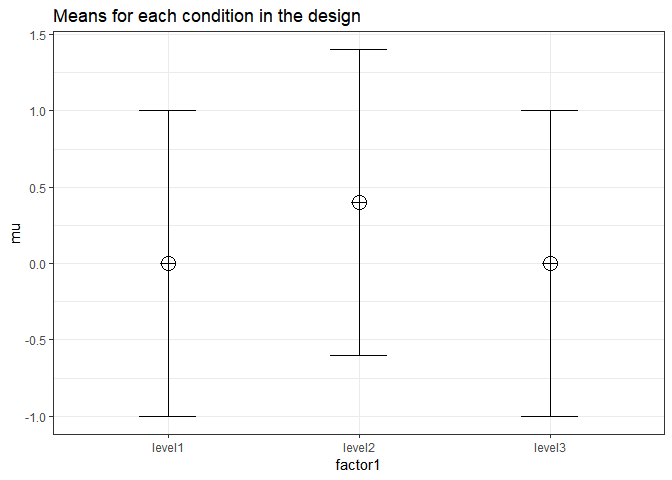
\includegraphics{1.3_validation_power_between_Brysbaert_1x3_files/figure-latex/unnamed-chunk-7-1.pdf}

\begin{Shaded}
\begin{Highlighting}[]
\KeywordTok{ANOVA_power}\NormalTok{(design_result, }\DataTypeTok{nsims =}\NormalTok{ nsims)}
\end{Highlighting}
\end{Shaded}

\begin{verbatim}
## Power and Effect sizes for ANOVA tests
##                power effect size
## anova_factor1 94.934      0.0368
## 
## Power and Effect sizes for contrasts
##                                  power effect size
## p_factor1_level1_factor1_level2 92.470      0.4016
## p_factor1_level1_factor1_level3  5.018      0.0004
## p_factor1_level2_factor1_level3 92.519     -0.4013
\end{verbatim}

\subsection{Variation 2}\label{variation-2}

\begin{Shaded}
\begin{Highlighting}[]
\CommentTok{# give sample sizes (all samples sizes are equal)}
\NormalTok{N =}\StringTok{ }\DecValTok{82}

\CommentTok{# give effect size d}
\NormalTok{d1 =}\StringTok{ }\FloatTok{.4} \CommentTok{#difference between the extremes}
\NormalTok{d2 =}\StringTok{ }\FloatTok{.2} \CommentTok{#third condition goes with the highest extreme}

\CommentTok{# give number of simulations}
\NormalTok{nSim =}\StringTok{ }\NormalTok{nsims}

\CommentTok{# give alpha levels}
\NormalTok{alpha1 =}\StringTok{ }\FloatTok{.05} \CommentTok{#alpha level for the omnibus ANOVA}
\NormalTok{alpha2 =}\StringTok{ }\FloatTok{.05} \CommentTok{#alpha level for three post hoc one-tailed t-tests Bonferroni correction}

\CommentTok{# create progress bar in case it takes a while}
\CommentTok{#pb <- winProgressBar(title = "progress bar", min = 0, max = nSim, width = 300)}

\CommentTok{# create vectors to store p-values}
\NormalTok{p1 <-}\KeywordTok{numeric}\NormalTok{(nSim) }\CommentTok{#p-value omnibus ANOVA}
\NormalTok{p2 <-}\KeywordTok{numeric}\NormalTok{(nSim) }\CommentTok{#p-value first post hoc test}
\NormalTok{p3 <-}\KeywordTok{numeric}\NormalTok{(nSim) }\CommentTok{#p-value second post hoc test}
\NormalTok{p4 <-}\KeywordTok{numeric}\NormalTok{(nSim) }\CommentTok{#p-value third post hoc test}
\NormalTok{pes1 <-}\KeywordTok{numeric}\NormalTok{(nSim) }\CommentTok{#partial eta-squared}
\NormalTok{pes2 <-}\KeywordTok{numeric}\NormalTok{(nSim) }\CommentTok{#partial eta-squared two extreme conditions}


\KeywordTok{library}\NormalTok{(lsr)}

\ControlFlowTok{for}\NormalTok{(i }\ControlFlowTok{in} \DecValTok{1}\OperatorTok{:}\NormalTok{nSim)\{ }\CommentTok{#for each simulated experiment}
 \CommentTok{# setWinProgressBar(pb, i, title=paste(round(i/nSim*100, 1), "% done"))}
\NormalTok{  x<-}\KeywordTok{rnorm}\NormalTok{(}\DataTypeTok{n =}\NormalTok{ N, }\DataTypeTok{mean =} \DecValTok{0}\NormalTok{, }\DataTypeTok{sd =} \DecValTok{1}\NormalTok{)}
\NormalTok{  y<-}\KeywordTok{rnorm}\NormalTok{(}\DataTypeTok{n =}\NormalTok{ N, }\DataTypeTok{mean =}\NormalTok{ d1, }\DataTypeTok{sd =} \DecValTok{1}\NormalTok{) }
\NormalTok{  z<-}\KeywordTok{rnorm}\NormalTok{(}\DataTypeTok{n =}\NormalTok{ N, }\DataTypeTok{mean =}\NormalTok{ d2, }\DataTypeTok{sd =} \DecValTok{1}\NormalTok{) }
\NormalTok{  data =}\StringTok{ }\KeywordTok{c}\NormalTok{(x,y,z)}
\NormalTok{  groups=}\StringTok{ }\KeywordTok{factor}\NormalTok{(}\KeywordTok{rep}\NormalTok{(letters[}\DecValTok{24}\OperatorTok{:}\DecValTok{26}\NormalTok{], }\DataTypeTok{each =}\NormalTok{ N))}
\NormalTok{  test <-}\StringTok{ }\KeywordTok{aov}\NormalTok{(data}\OperatorTok{~}\NormalTok{groups)}
\NormalTok{  pes1[i] <-}\StringTok{ }\KeywordTok{etaSquared}\NormalTok{(test)[}\DecValTok{1}\NormalTok{,}\DecValTok{2}\NormalTok{]}
\NormalTok{  p1[i] <-}\StringTok{ }\KeywordTok{summary}\NormalTok{(test)[[}\DecValTok{1}\NormalTok{]][[}\StringTok{"Pr(>F)"}\NormalTok{]][[}\DecValTok{1}\NormalTok{]]}
\NormalTok{  p2[i] <-}\StringTok{ }\KeywordTok{t.test}\NormalTok{(x,y)}\OperatorTok{$}\NormalTok{p.value}
\NormalTok{  p3[i] <-}\StringTok{ }\KeywordTok{t.test}\NormalTok{(x,z)}\OperatorTok{$}\NormalTok{p.value}
\NormalTok{  p4[i] <-}\StringTok{ }\KeywordTok{t.test}\NormalTok{(y,z)}\OperatorTok{$}\NormalTok{p.value}
\NormalTok{  data =}\StringTok{ }\KeywordTok{c}\NormalTok{(x,y)}
\NormalTok{  groups=}\StringTok{ }\KeywordTok{factor}\NormalTok{(}\KeywordTok{rep}\NormalTok{(letters[}\DecValTok{24}\OperatorTok{:}\DecValTok{25}\NormalTok{], }\DataTypeTok{each =}\NormalTok{ N))}
\NormalTok{  test <-}\StringTok{ }\KeywordTok{aov}\NormalTok{(data}\OperatorTok{~}\NormalTok{groups)}
\NormalTok{  pes2[i] <-}\StringTok{ }\KeywordTok{etaSquared}\NormalTok{(test)[}\DecValTok{1}\NormalTok{,}\DecValTok{2}\NormalTok{]}
\NormalTok{  \}}
\CommentTok{#close(pb)#close progress bar}

\CommentTok{# results are as predicted when omnibus ANOVA is significant, t-tests are significant between x and y plus x and z; not significant between y and z}
\CommentTok{#printing all unique tests (adjusted code by DL)}
\KeywordTok{sum}\NormalTok{(p1}\OperatorTok{<}\NormalTok{alpha1)}\OperatorTok{/}\NormalTok{nSim}
\end{Highlighting}
\end{Shaded}

\begin{verbatim}
## [1] 0.62062
\end{verbatim}

\begin{Shaded}
\begin{Highlighting}[]
\KeywordTok{sum}\NormalTok{(p2}\OperatorTok{<}\NormalTok{alpha2)}\OperatorTok{/}\NormalTok{nSim}
\end{Highlighting}
\end{Shaded}

\begin{verbatim}
## [1] 0.72328
\end{verbatim}

\begin{Shaded}
\begin{Highlighting}[]
\KeywordTok{sum}\NormalTok{(p3}\OperatorTok{<}\NormalTok{alpha2)}\OperatorTok{/}\NormalTok{nSim}
\end{Highlighting}
\end{Shaded}

\begin{verbatim}
## [1] 0.24965
\end{verbatim}

\begin{Shaded}
\begin{Highlighting}[]
\KeywordTok{sum}\NormalTok{(p4}\OperatorTok{<}\NormalTok{alpha2)}\OperatorTok{/}\NormalTok{nSim}
\end{Highlighting}
\end{Shaded}

\begin{verbatim}
## [1] 0.24593
\end{verbatim}

\begin{Shaded}
\begin{Highlighting}[]
\KeywordTok{mean}\NormalTok{(pes1)}
\end{Highlighting}
\end{Shaded}

\begin{verbatim}
## [1] 0.03390686
\end{verbatim}

\begin{Shaded}
\begin{Highlighting}[]
\KeywordTok{mean}\NormalTok{(pes2)}
\end{Highlighting}
\end{Shaded}

\begin{verbatim}
## [1] 0.04428841
\end{verbatim}

\subsection{Three conditions
replication}\label{three-conditions-replication-2}

\begin{Shaded}
\begin{Highlighting}[]
\NormalTok{K <-}\StringTok{ }\DecValTok{3}
\NormalTok{mu <-}\StringTok{ }\KeywordTok{c}\NormalTok{(}\DecValTok{0}\NormalTok{, }\FloatTok{0.4}\NormalTok{, }\FloatTok{0.2}\NormalTok{)}
\NormalTok{n <-}\StringTok{ }\DecValTok{82}
\NormalTok{sd <-}\StringTok{ }\DecValTok{1}
\NormalTok{string =}\StringTok{ }\KeywordTok{paste}\NormalTok{(K,}\StringTok{"b"}\NormalTok{,}\DataTypeTok{sep=}\StringTok{""}\NormalTok{)}
\end{Highlighting}
\end{Shaded}

\begin{Shaded}
\begin{Highlighting}[]
\NormalTok{design_result <-}\StringTok{ }\KeywordTok{ANOVA_design}\NormalTok{(}\DataTypeTok{string =}\NormalTok{ string,}
                   \DataTypeTok{n =}\NormalTok{ n, }
                   \DataTypeTok{mu =}\NormalTok{ mu, }
                   \DataTypeTok{sd =}\NormalTok{ sd, }
                   \DataTypeTok{labelnames =} \KeywordTok{c}\NormalTok{(}\StringTok{"factor1"}\NormalTok{, }\StringTok{"level1"}\NormalTok{, }\StringTok{"level2"}\NormalTok{, }\StringTok{"level3"}\NormalTok{))}
\end{Highlighting}
\end{Shaded}

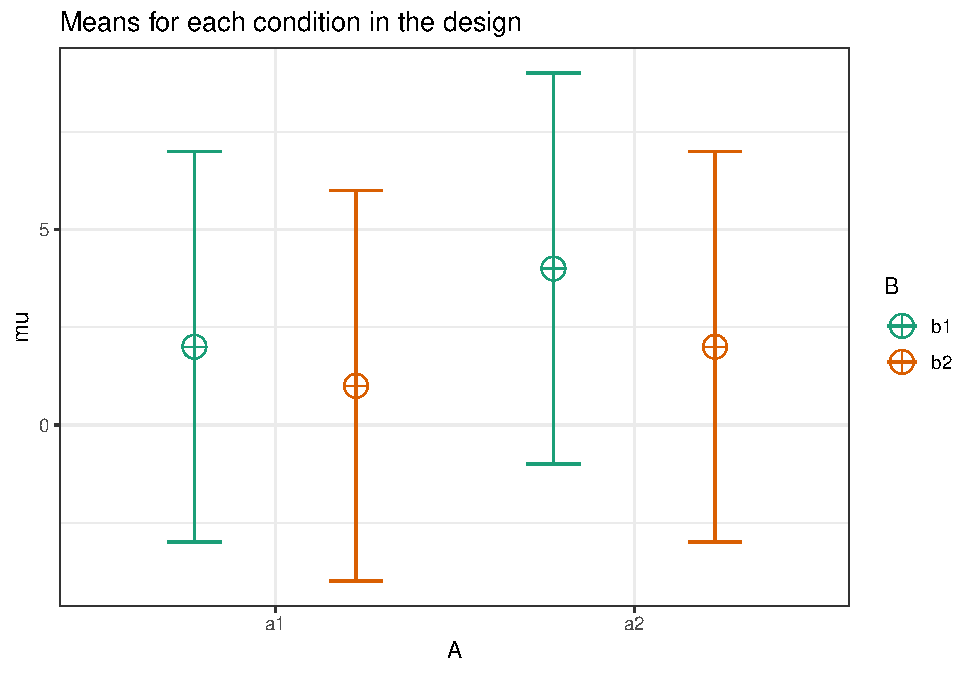
\includegraphics{1.3_validation_power_between_Brysbaert_1x3_files/figure-latex/unnamed-chunk-10-1.pdf}

\begin{Shaded}
\begin{Highlighting}[]
\KeywordTok{ANOVA_power}\NormalTok{(design_result, }\DataTypeTok{nsims =}\NormalTok{ nsims)}
\end{Highlighting}
\end{Shaded}

\begin{verbatim}
## Power and Effect sizes for ANOVA tests
##                power effect size
## anova_factor1 61.943      0.0304
## 
## Power and Effect sizes for contrasts
##                                  power effect size
## p_factor1_level1_factor1_level2 72.179      0.4022
## p_factor1_level1_factor1_level3 24.520      0.2007
## p_factor1_level2_factor1_level3 24.731     -0.2015
\end{verbatim}


\end{document}
